\documentclass[10pt,letterpaper]{article}
\usepackage{fullpage}
\usepackage[top=2cm, bottom=4.5cm, left=2.5cm, right=2.5cm]{geometry}
\usepackage{amsmath,amsthm,amsfonts,amssymb,amscd}
\usepackage{lastpage}
\usepackage{enumerate}
\usepackage{empheq}
\usepackage{fancyhdr}
\usepackage{mathrsfs}
\usepackage{mathtools}
\usepackage{xcolor}
\usepackage{graphicx}
\usepackage{caption}
\usepackage{listings}
\usepackage{hyperref}
\usepackage{pifont}
\newcommand{\xmark}{\ding{55}}%
\pagestyle{fancyplain}
\headheight 25pt
\lhead{LOGAN CAMPBELL \\ Discrete Mathematics : Lecture Notes (9/23/2019)}
\chead{}
\lfoot{}
\cfoot{}
\rfoot{\small\thepage}
\headsep 1.0em
\begin{document}
{
    \begin{enumerate}
    \item[]Let $A$ and $B$ be sets:
    
    union ( $\cup$ ) \quad $\cdot \quad \cdot$ $A \cup B := \{x : x \in A $ or $x \in B \}$
    
    intersection ( $\cap$ ) \quad $\cdot \quad \cdot$ $A \cap B := \{x : x \in A $ and $x \in B \}$
    
    set difference ( $\setminus$ ) \quad $\cdot \quad \cdot$ $A \setminus B := \{x : x \in A $ and $x \not \in B \}$
    
    symmetric difference ( $\bigtriangleup $ ) \quad $\cdot \quad \cdot$ $A \bigtriangleup B := \{ (A \setminus B) \cup (B\setminus A) \}$
    
    \subsection*{Example}
    Let $A - \{-5,0,7\}$ and let $B = \{-\pi, 0, 8 \}$ \qquad $\therefore$
    $$\cdot \quad A \cup B = \{ -\pi, -5, 0,7,8 \} \quad \checkmark$$
    $$\cdot \quad A \cap B = \{ 0 \} \quad \checkmark$$
    $$\cdot \quad A \setminus B = \{ -5,7 \} \quad \checkmark $$
    $$\cdot \quad B \setminus B = \{ -\pi, 8\} \quad \checkmark$$
    $$\cdot \quad A \bigtriangleup B = \{ -5,7,-\pi, 8 \} \quad \checkmark $$ 
    \hrule
    \end{enumerate}
    
    % \newpage{}
    \begin{enumerate}
        \item [] 
        $$ \mathbb{R}^{2}   = \mathbb{R} \times \mathbb{R} $$
        $$\{ (x_{2}, x_{1}) : x_{1} \in \mathbb{R} \ and \ x_{2} \in \mathbb{R} \} $$
        Illustration:
        \begin{center}
                    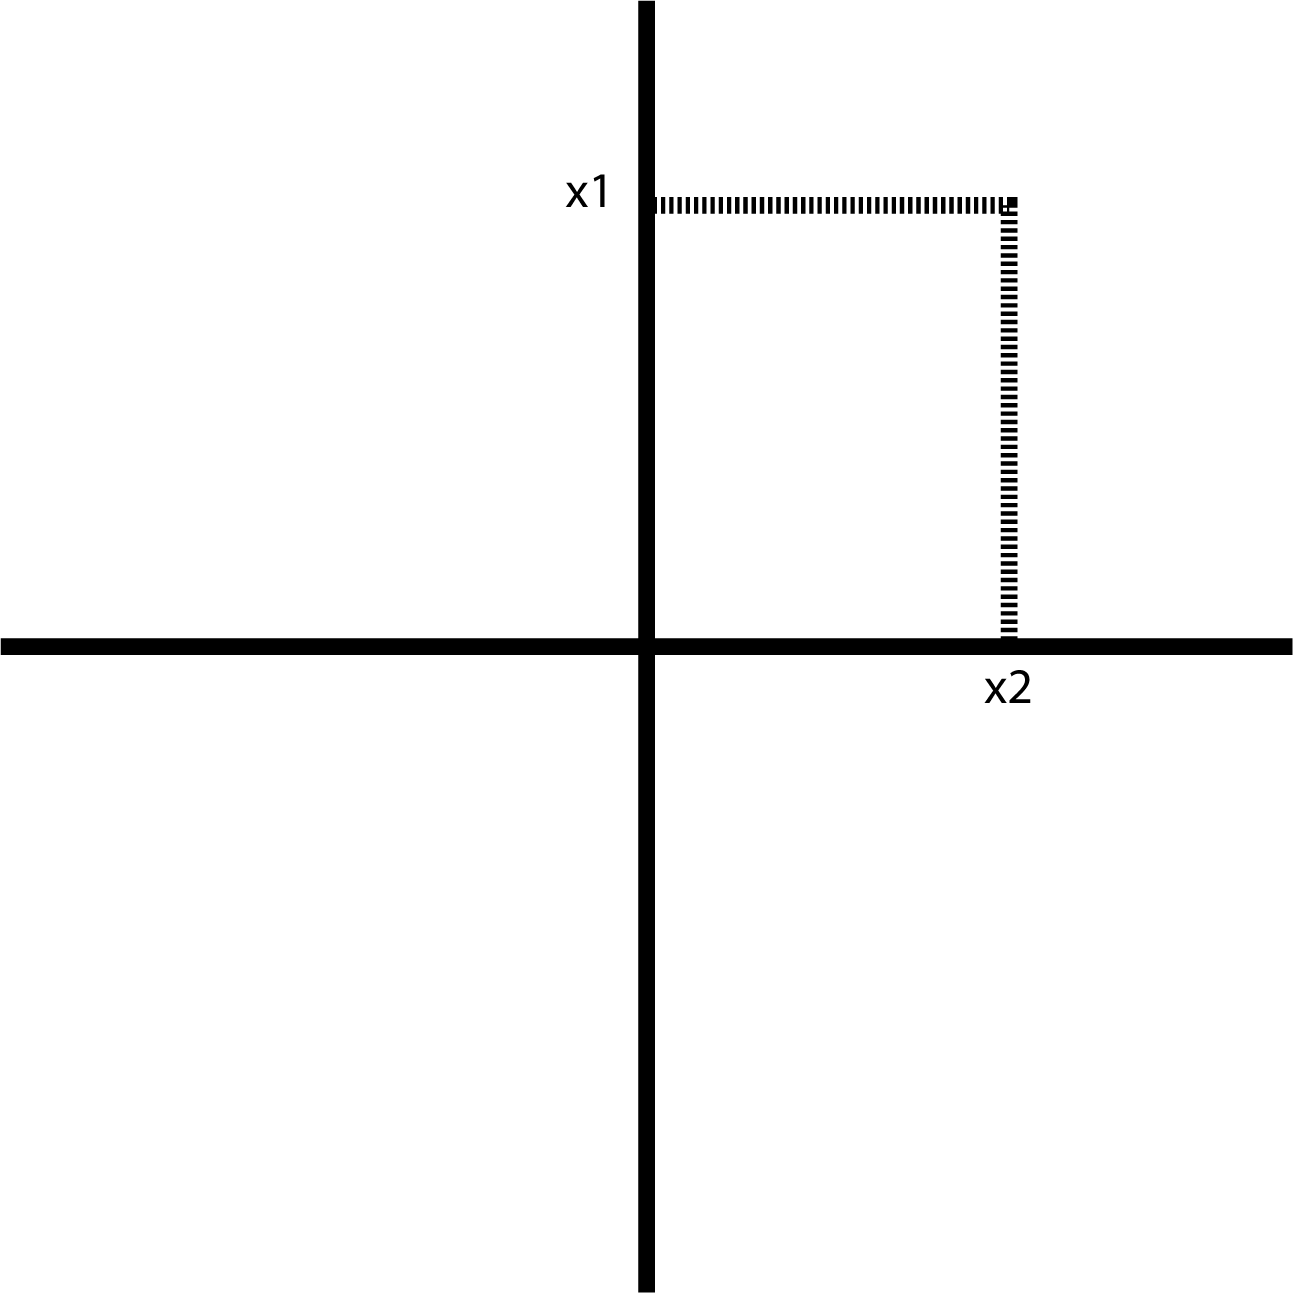
\includegraphics[scale = .5]{illustrations/x1x2graph.png}

        \end{center}
        
    \end{enumerate}
    
    Definition: Let A, B, and C be non empty sets.
    
    The Cartesian product of A with B 
    $$ A \times B = \{ (a,b) : a \in A \text{ and } b \in B\}$$ 
    \quad (NOTE: $\mathbb{R} \times \mathbb{R} = \mathbb{R}^{2} \leftarrow$ Cartesian Plane)
    
    Cartesian Product of A,B,C : $A \times B \times C = \{ (a,b,c) = a \in A, b \in B, c \in C \}$
    \vspace{.4em}
    \hrule
    \vspace{.4em}

    Example:
    $$ A = \{ 1,2\} \quad B = \{a,b\} \quad C = \{\alpha,\beta\} $$
    $$ \cdot  \qquad A \times B = \{(1,a), (1,b), (2,A), (2,b)\}$$
        
    $$ \cdot  \qquad A \times B \times C = \{(1,a,\alpha), (1,a,\beta), (1,b,\alpha), (1,b,\beta), (2,a,\alpha), (2,a,\beta),(2,b,\alpha), (2,b,\beta) \}$$
    
    NOTICE : The number of elements times each  other $\rightarrow |A| \cdot |B| \cdot |C| = |A\times B\times C|$
    
    \newpage
    \begin{enumerate}
        \item [] 
        Two sets are to be disjoint if for an example: sets $A$ and $B$ are intersection with each other $A \cap B$ and the outcome is the empty set $\therefore A \cap B = \emptyset$.
        
        Pair
        
        A collection of sets $\{A_{1},A_{2},\ldots,A_{n} \} $ is called a Partition of set $\mathcal{X}$
        if:
        $$ A_{i} \not = \emptyset \text{ for i = 1,2,3...n}$$ 
        $$ \{A_{1},A_{2},\ldots,A_{n}\} \text{ is a pairwise disjoint collection }$$
        $$ \mathcal{X} = A_{1} \cup A_{2} \cup A_{3} \cup \ldots \cup A_{n} $$
        
        
    \end{enumerate}{}
}
\end{document}
